\chapter{Filesystem}
\section{Introduction}
For the filesystem, we support SD-cards running FAT32. The filesystem we've implemented 
is built as a service, exposing RPC calls for file operations like opening, closing, writing, reading, etc. 
to user processes, which then can be called by the usual libc functions like \texttt{fopen}, \texttt{fclose}, \texttt{fwrite}.

The alternative, which is building the filesystem as a library, has not be chosen because the filesystem as a service in our eyes
gives a better abstraction to the underlying FAT32 operations. Another reason why we chose the filesystem as a service
is because it does decrease RPC communication, leading to overall better performance. Probably most importantly, given processes
access to read/write functionality of the block driver leads to a decentralized filesystem state, where it is not clear how to easily
add thread safety as well as gather information about which file handles are opened where efficiently.

\subsection{Operations}
The operations implemented as a service over RPC calls are:
\begin{itemize}
    \item \texttt{aos\_rpc\_fs\_open}: Open a file with given flags
    \item \texttt{aos\_rpc\_fs\_close}: Close a file
    \item \texttt{aos\_rpc\_fs\_create}: Create a file
    \item \texttt{aos\_rpc\_fs\_read}: Read open file contents into buffer
    \item \texttt{aos\_rpc\_fs\_write}: Write buffer contents to a open file
    \item \texttt{aos\_rpc\_fs\_lseek}: Seeking in a file
    \item \texttt{aos\_rpc\_fs\_dir\_action}: Used to perform the two operations \texttt{mkdir}, \texttt{rmdir}
    \item \texttt{aos\_rpc\_fs\_readdir}: Read directory contents
    \item \texttt{aos\_rpc\_fs\_fstat}: Get file status
\end{itemize}

\section{Block Driver}
After flashing a new filesystem onto the SD-card, we can communicate with it over 
the block driver over the process \texttt{fs}, which has access to the devframe necessary
for using the driver. Since it's the only process with access to the SD-card, we don't have to worry 
about concurrent read/writes in the filesystem.

\subsection{Performance Improvements}
To improve the block driver, we note that we always only read/write blocks of the 
same size with it. Thus, it's enough to only set the block-size once in the beginning,
instead of setting it every time we read/write a block. As we will see during the 
performance analysis in the next section, this will already give a 2x speedup.

There are many other performance improvements which could be made.
Very interestingly to me with respect to FAT32 is that reading/writing whole 
clusters at once could be done much faster. As can be seen in the next section,
sending commands over the block driver alone will take a lot of time, 
so reducing the number of commands sent to the block driver can be of essential 
importance for performance.

It's also possible to read/write specific block-lengths with each write.
However, this change in block-lengths needs to be communicated to the device,
thus another command needs to be send to the SD-reader. We immediately see 
that this constitutes a trade-off between send-commands and DMA-access time.
While always reading large blocks has few send-commands, DMA over large memory 
takes longer than for small blocks. It could have been interesting to also 
check if or at which point it makes sense to work with variable-sized read/write 
commands.

As a last possibility for improving performance, it could have been possible 
to fetch information from the SD-card to obtain more information of frequencies 
which could be used to allow for faster access speed.

\subsection{Performance Analysis}
\begin{figure}[h]
    \centering
    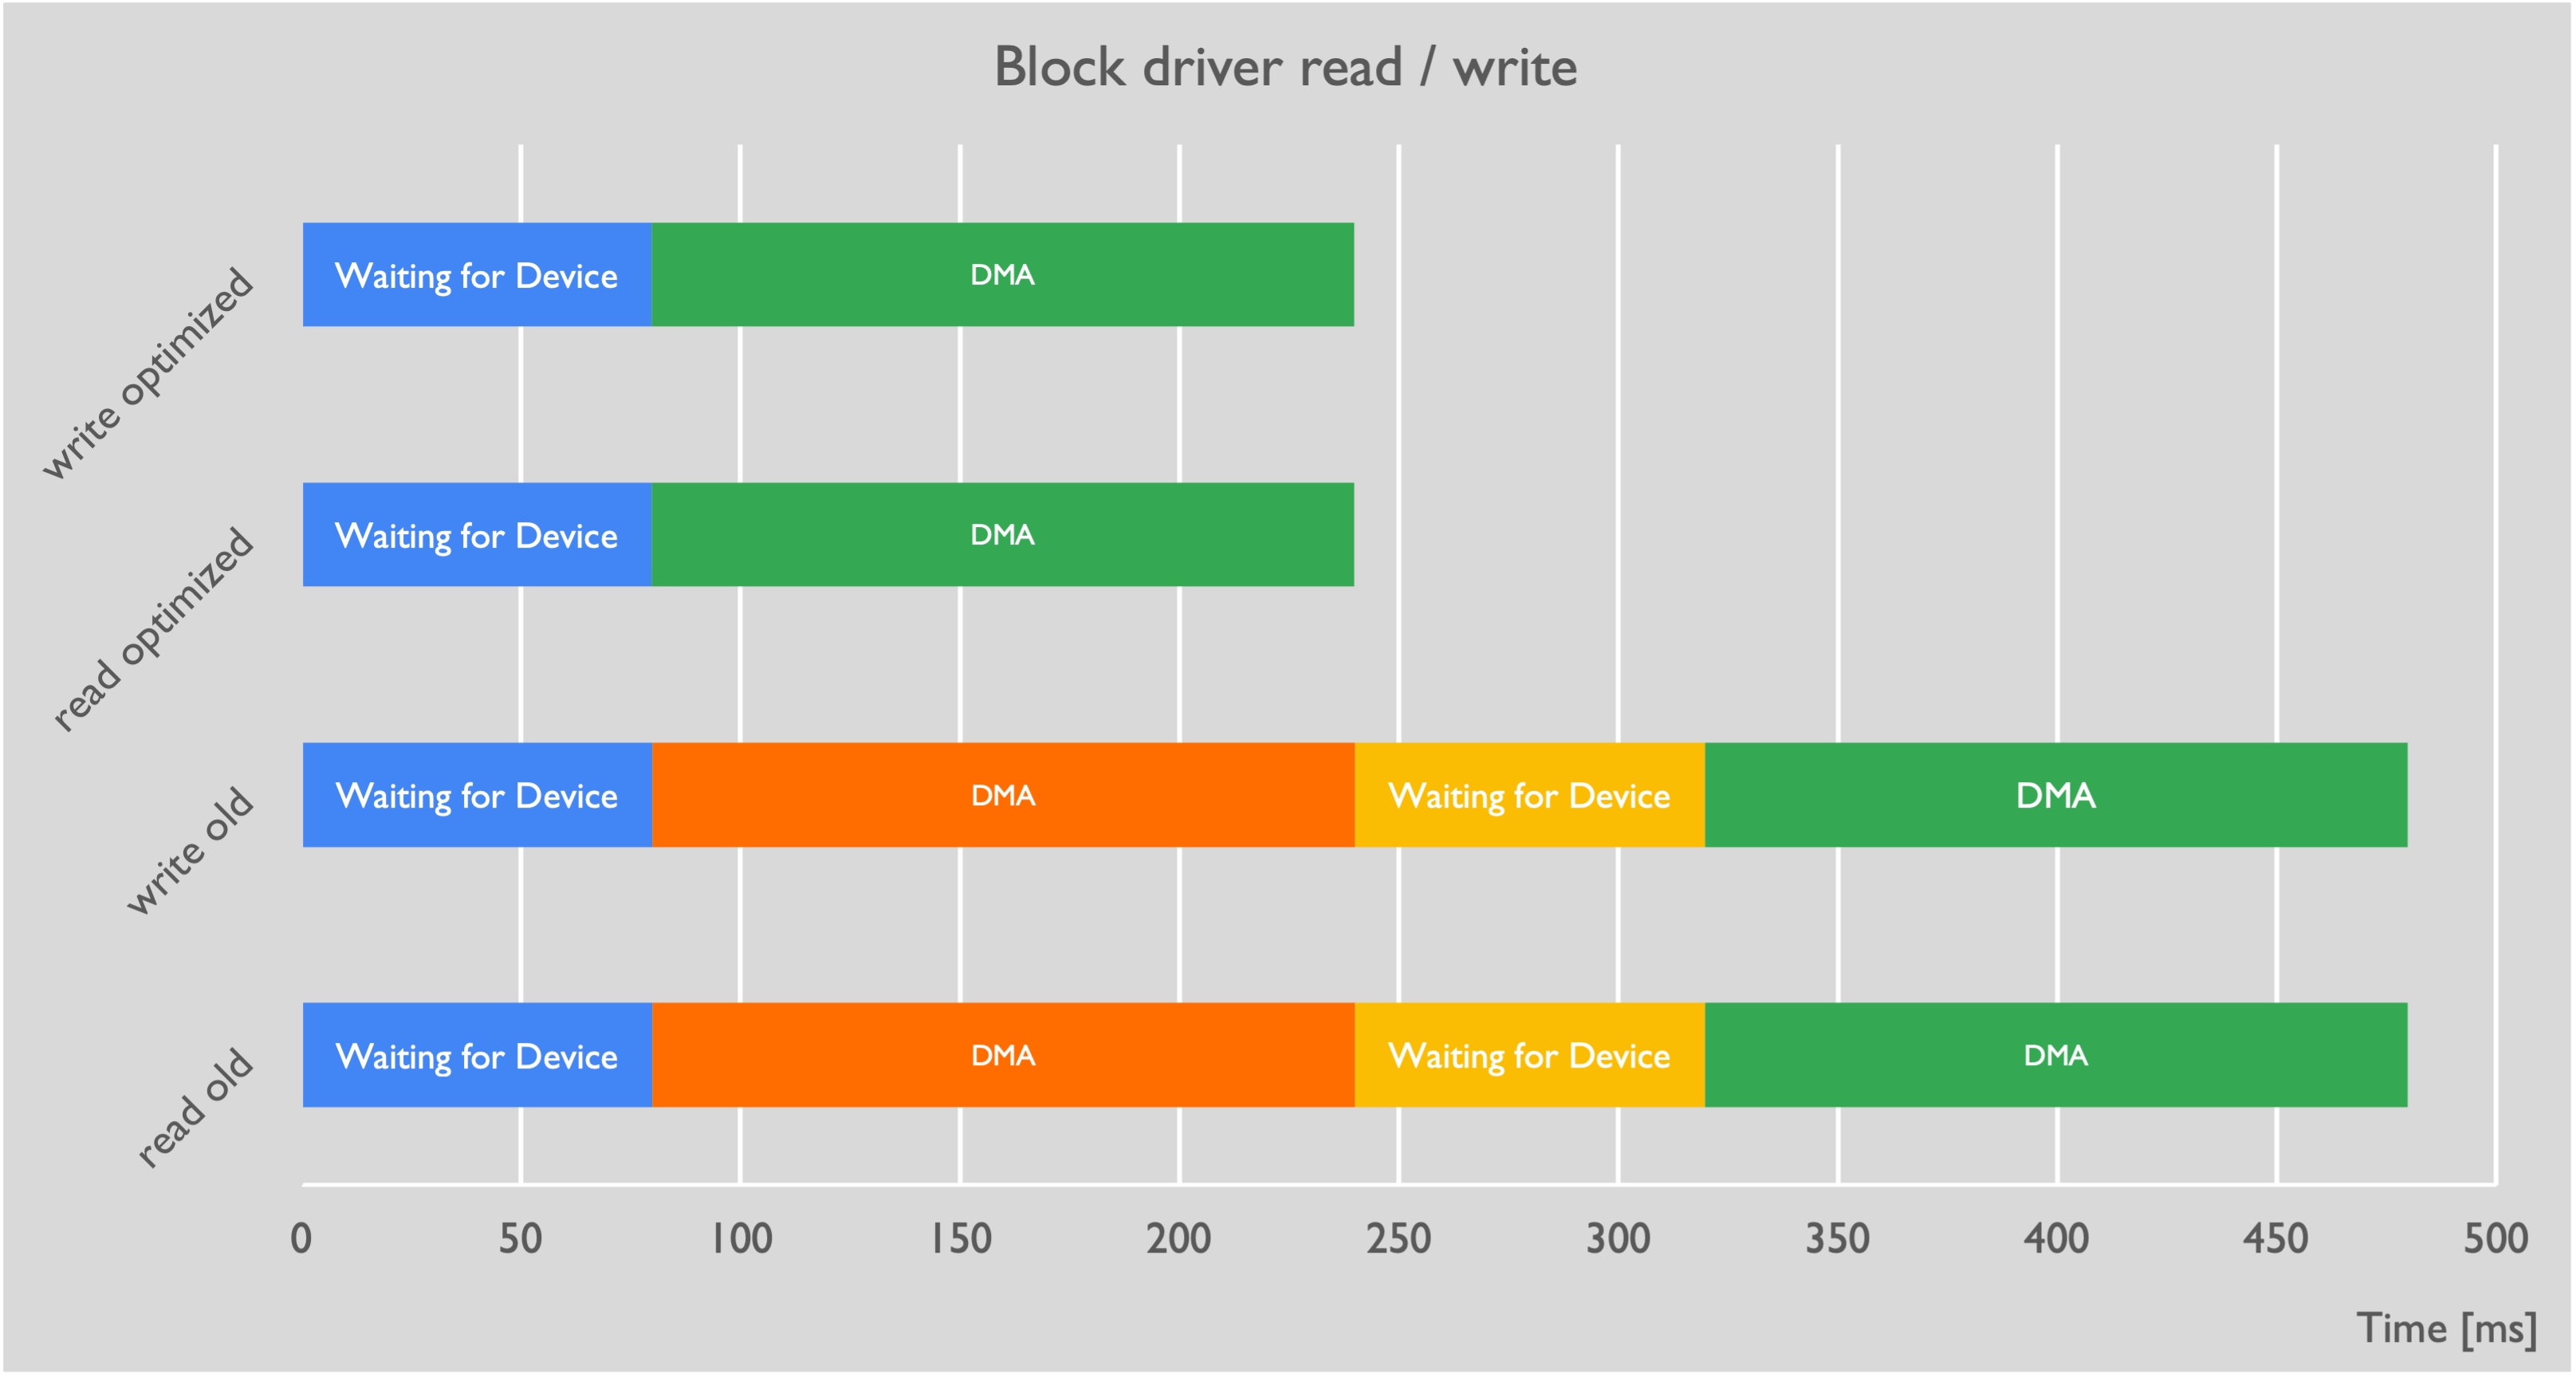
\includegraphics[scale=0.5]{block_driver.png}
    \caption{Read/Write Bandwidth with and without caching}
    \label{fig:block_driver}
\end{figure}

In Figure~\ref{fig:block_driver}, we measured averages of block read and write operations over 50 requests and compared the optimized version with 
the unoptimized one. We can see that the optimization of removing the first command to the SD-card (which sets the block-length)
halves the latency of a read and write request. Furthermore, we see that waiting for the device and the following DMA requests
all take roughly the same amount of time.
In total, the optimized version achieved a latency of 0.239s for 512 bytes, which leads to a bandwidth of 2142B/s. The write bandwidth
takes the same amount of time.
\section{FAT32 Implementation}

\subsection{Assumptions}
We assume we receive a valid FAT32 filesystem. We thus don't do any additional 
checking/fixing/infering of the filesystem present.
We furthermore don't implement thread-safety features into the FAT32 implementation.
Thread-safety will be the task of the filesystem which builds ontop of this.

\subsection{Abstractions}
Wherever possible, we tried to abstract away sectors as much as possible.
Instead, we focused on clusters and indeces into clusters, so that 
we wouldn't have to worry too much about cluster traversals in terms of 
sectors, where in which cluster we are, etc. Seeing FAT32 as a linked-list 
of clusters is much easier than seeing it as a linked-list of sector-arrays.

The sdhc driver uses DMA request, for which we need buffers and their 
physical addresses. We also need to take care that caches are flushed
before reads/writes, to stay consistent.
For the buffers which we use to read/write to, we introduced:

\begin{minted}{c}
struct phys_virt_addr {
    // physical address of memory segment
    lpaddr_t phys;
    // virtual address of memory segment
    void *virt;
    // last sector read/written
    uint32_t last_sector;
    // is the buffer dirty?
    bool dirty;
};
\end{minted}
which we use to keep track of where we read/write to.
The last two members are important for caching, which is another big abstraction we make over the FAT32 implementation
and will be explained later.

\section{Directories}
Directories contain directory entries, holding meta data for it's contained files and directories like names, sizes, data location, etc.
Each directory entry is 32 bytes in size. We didn't implement long file names, so each directory entry has a fixed size.
The FAT32 specification contains many small details which are important. For example, when creating a new directory, all directory entries
of their clusters must be zeroed out. For performance, one could store a flag into the last directory entry, so that none of the remaining
entries in the cluster need to be looked at when looking for particular files. We didn't implement this feature, however concerning the block 
driver speed, this would be a major performance increase for \texttt{readdir}.

Since every new directory contains the two directories "." (dot) and ".." (dotdot), it is trivial to use those for moving back to a parent directory
as well as receive information about the current directory. 

\section{Traversing a Linked List}
Next to reading/writing directory entries, the functionality required to a minimal implementation of FAT32 as per specification is the reading/writing of data clusters containing the data of a file. As known, the data is structured as a linked list of data clusters, where next blocks can be looked up in the 
in the File Allocation Table (FAT). Reading/writing files is then only a matter of traversing linked lists, while continuously reading/writing
the clusters, which represent a single node in the linked list. One has to be careful to assign the EOF flag to FAT entries as well as not overriding
the top bits of a FAT entry, which are reserved. 

Thus, for writing a file, one has to read/write to the directory entry itself (to keep track of the file size), the FAT for reading/writing next-pointers
in the linked list, as well as the data clusters itself. Many sectors are touched during these operations.

\section{Caching}
One file write/read can potentially look at one FAT-sector multiple times,
or could write to the same data sector multiple times. Since every 
read/write from/to a sector on the SD-card is very expensive, a big 
performance increase was the idea of caching reads/writes to the disk, in memory.

In a first attempt, we never performed a read from the SD-card if 
the last read/write to/from the SD-card was to the same sector. This can 
be pretty easily by just remembering the last sector each time.

A next observation was that there is much locality in a directory-entry 
as well as a FAT-sector, since many requests looked at closed-by indeces
of a sector. For that reason, we decided to use a different buffer 
for storing any read/writes to a data-sector and a different one for 
FAT sectors (and directory-entry-sectors). 
A write would still always write, it is write-through.

Using these two different buffer, we benefit from locality.
To extend this idea even further, an LRU-approach with $N$ different 
buffers would lead to even fewer reads/writes from/to the SD-card.

\subsection{Limitations}
Due to time-constraints, no support for timestamps or read-only files is implemented.
Also, no estimates of free clusters are used. As previously state, we also didn't specify if a directory entry in a cluster is the last 
overall directory entry. Read-only flags are ignored and no support was added for designating files as read-only.
We also only use the first of the two File Allocation Tables.

\section{Filesystem Implementation}

\subsection{Requirements}
As said already, our filesystem is a filesystem as a service.
\begin{itemize}
    \item The filesystem is accessible for any user thread which has the \texttt{fs} library loaded
    \item The filesystem is responsible for thread-safety under the assumption that the underlying FAT32 implementation is not thread-safe
    \item It must keep track of any open file/directory in the whole system
    \item It should implement all the functions in \texttt{lib/fs/fopen.c} and \texttt{lib/fs/dirent.c} as to abstract the implementation from the use
\end{itemize}



\subsection{Approach}
For these requirements, the filesystem service is provided by a user process called \texttt{fs}.
This process handles all the requests to the filesystem using RPC. It is registered over the nameserver with the name \texttt{fs} and 
over that reacheable from any other user process. One subtlety is that the \texttt{fs} process itself can't use the filesystem over the same 
functions as the client (i.e. \texttt{fopen} won't work). The filesystem implements the RPC functions specified in the beginning of this chapter.

The other side of the implementation is the client side, which abstracts away the service using functions like \texttt{fopen, fclose}, etc.

To implement the client-side of the filesystem, we tried to keep the original approach of \texttt{ramfs}
as much as possible and replaced functions like \texttt{ramfs\_open}, \texttt{ramfs\_close}
by \texttt{aos\_rpc\_fs\_open}, \texttt{aos\_rpc\_fs\_close}, etc.

We store a opened file/directory in a similiar manner as in \texttt{ramfs}:

\begin{minted}{c}
struct fat32fs_dirent {
    char *name; 
    size_t size; 
    bool is_dir; 
    // cluster containing the directory-entry
    uint32_t dir_cluster; 
    // index into that cluster
    uint32_t dir_index; 
    // first data cluster of file
    uint32_t start_data_cluster; 
};

struct fat32fs_handle {
    int flags;
    // unique id of the opened file
    fileref_id_t fid;
    domainid_t pid;
    char *path;
    struct fat32fs_dirent *dirent;
    union {
        uint32_t dir_offset;
        uint32_t file_offset;
    } u;
    // current data cluster as 
    // specified by dir_offset/file_offset
    uint32_t curr_data_cluster;
};
\end{minted}
Of particular importance is the member \texttt{fid}.
This ID is a unique ID under all the opened files in the filesystem 
which is used to identify an opened handle in the \texttt{fs} process. Any RPC request to an opened
file identifies the handle uniquely by this FID. The FID is a global file descriptor, which is abstracted away in client processes.
Client requests to open file send this FID to talk to the service.

\subsubsection{Server Side}
The server side of the filesystem is implemented in \texttt{lib/fs/fat32fs.c} and builds on top of the FAT32 implementation.
In the \texttt{fs} process, the following happens when a new file/dir is opened:
\begin{itemize}
    \item Create new handle, store file-info into it
    \item Assign new unique FID to handle
    \item Add into hashmap \texttt{fid2handle}, which maps FID's to handles
    \item Append to hashmap \texttt{path2handle}, which maps a file path to a list of opened handles to that file
\end{itemize}
The first of the two hashmaps is used to find the handle of an opened file by FID in constant 
time. Using this second hash map, we resolve many thread-safety issues, which will be explained later.

On top of \texttt{fat32fs}, we register a nameservice called \texttt{fs} and with that a handler which responds to client requests.
This handler can be found in \texttt{lib/fs/fs\_rpc.c}.
Other than responding to requests, it has another important task: Thread Safety.
\subsection{Thread Safety}
To ensure two threads (or two processes) which access the same time can fulfill their requests, we implemented thread safety on top 
of the RPC handler in combination with the two hashmaps \texttt{path2handle, fid2handle}, which was mentioned previously.
Note first that most problems concerning thread safety are resolved already by locking on receival of a request and unlocking when
processing is done. 
Problems which are not resolved by that is anything that changes state in the handler itself. This includes for example:
\begin{itemize}
    \item Files can be requested to be deleted when they are opened somewhere else.
    \item When one processes increases the a file's size, this new size must be updated in the other open handles
    \item When one process decreases a file's size, the current file offsets of other opened handles to the same file might become invalid.
    \item 2 processes attempt to wrie to the same offset of the same file 
\end{itemize}
As a solution to those problems, we do the following.
\begin{itemize}
    \item Whenever a file is to be deleted but is already open, we deny the request.
    \item When a file size increases (due to new content written), we update all the other open handles to that file using the bookkeeping in \texttt{path2handle}
    \item Should a file size be decreased, we update any file offsets to other handles which are now out of bound to the end of the new file size.
    \item For writes to the same file, it is enough to handle them atomically by locking. Thus, both offsets will be written, but one of them 
    will overwrite the progress of the other one.
\end{itemize}

For processes which write to the same file offset on a same file, the result will be that both requests are fulfilled, however
after the first has been handled, the second will overwrite it. This has to be kept in mind by the programmer in userspace and is
not handled any further in the OS.

When a process changes the size of a file, we use the hashmap \texttt{path2fid} to update all handles which have the same file opened.
In addition, should a file size change, 

\subsection{Security}
For a full-blown OS, it makes sense to have a security layer in place which 
doesn't allow for one process to read/write using FID's of another process.
This could have been done in multiple ways. One could be to authenticate the RPC channels,
so that every FID is also linked to a specific channel. That way, requests to foreign 
FID's could be rejected. This could also have been done with special capabilities to
any opened file/directory. 

As this feature was of rather low priority given the mentioned problems we had during the integration, no additional security feature was implemented.

\section{ELF Loading}
Due to the problems during integration-phase, we didn't have time to implement
the ELF loading feature.

However, for the sake of completeness, we now state how this would be achieved.
Given our existing code, the approach we would follow is to use 
the file system to load the complete file into memory. After that,
any arguments to the program would be passed to by the shell.
To actually load the in-memory program, we can use existing functionality 
we have in our \texttt{spawn} library, where multiboot programs 
are also loaded into memory. After this step, we would start the program 
in the same way as we did for any other program.

\section{Performance Analysis}

\begin{figure}[h]
\centering
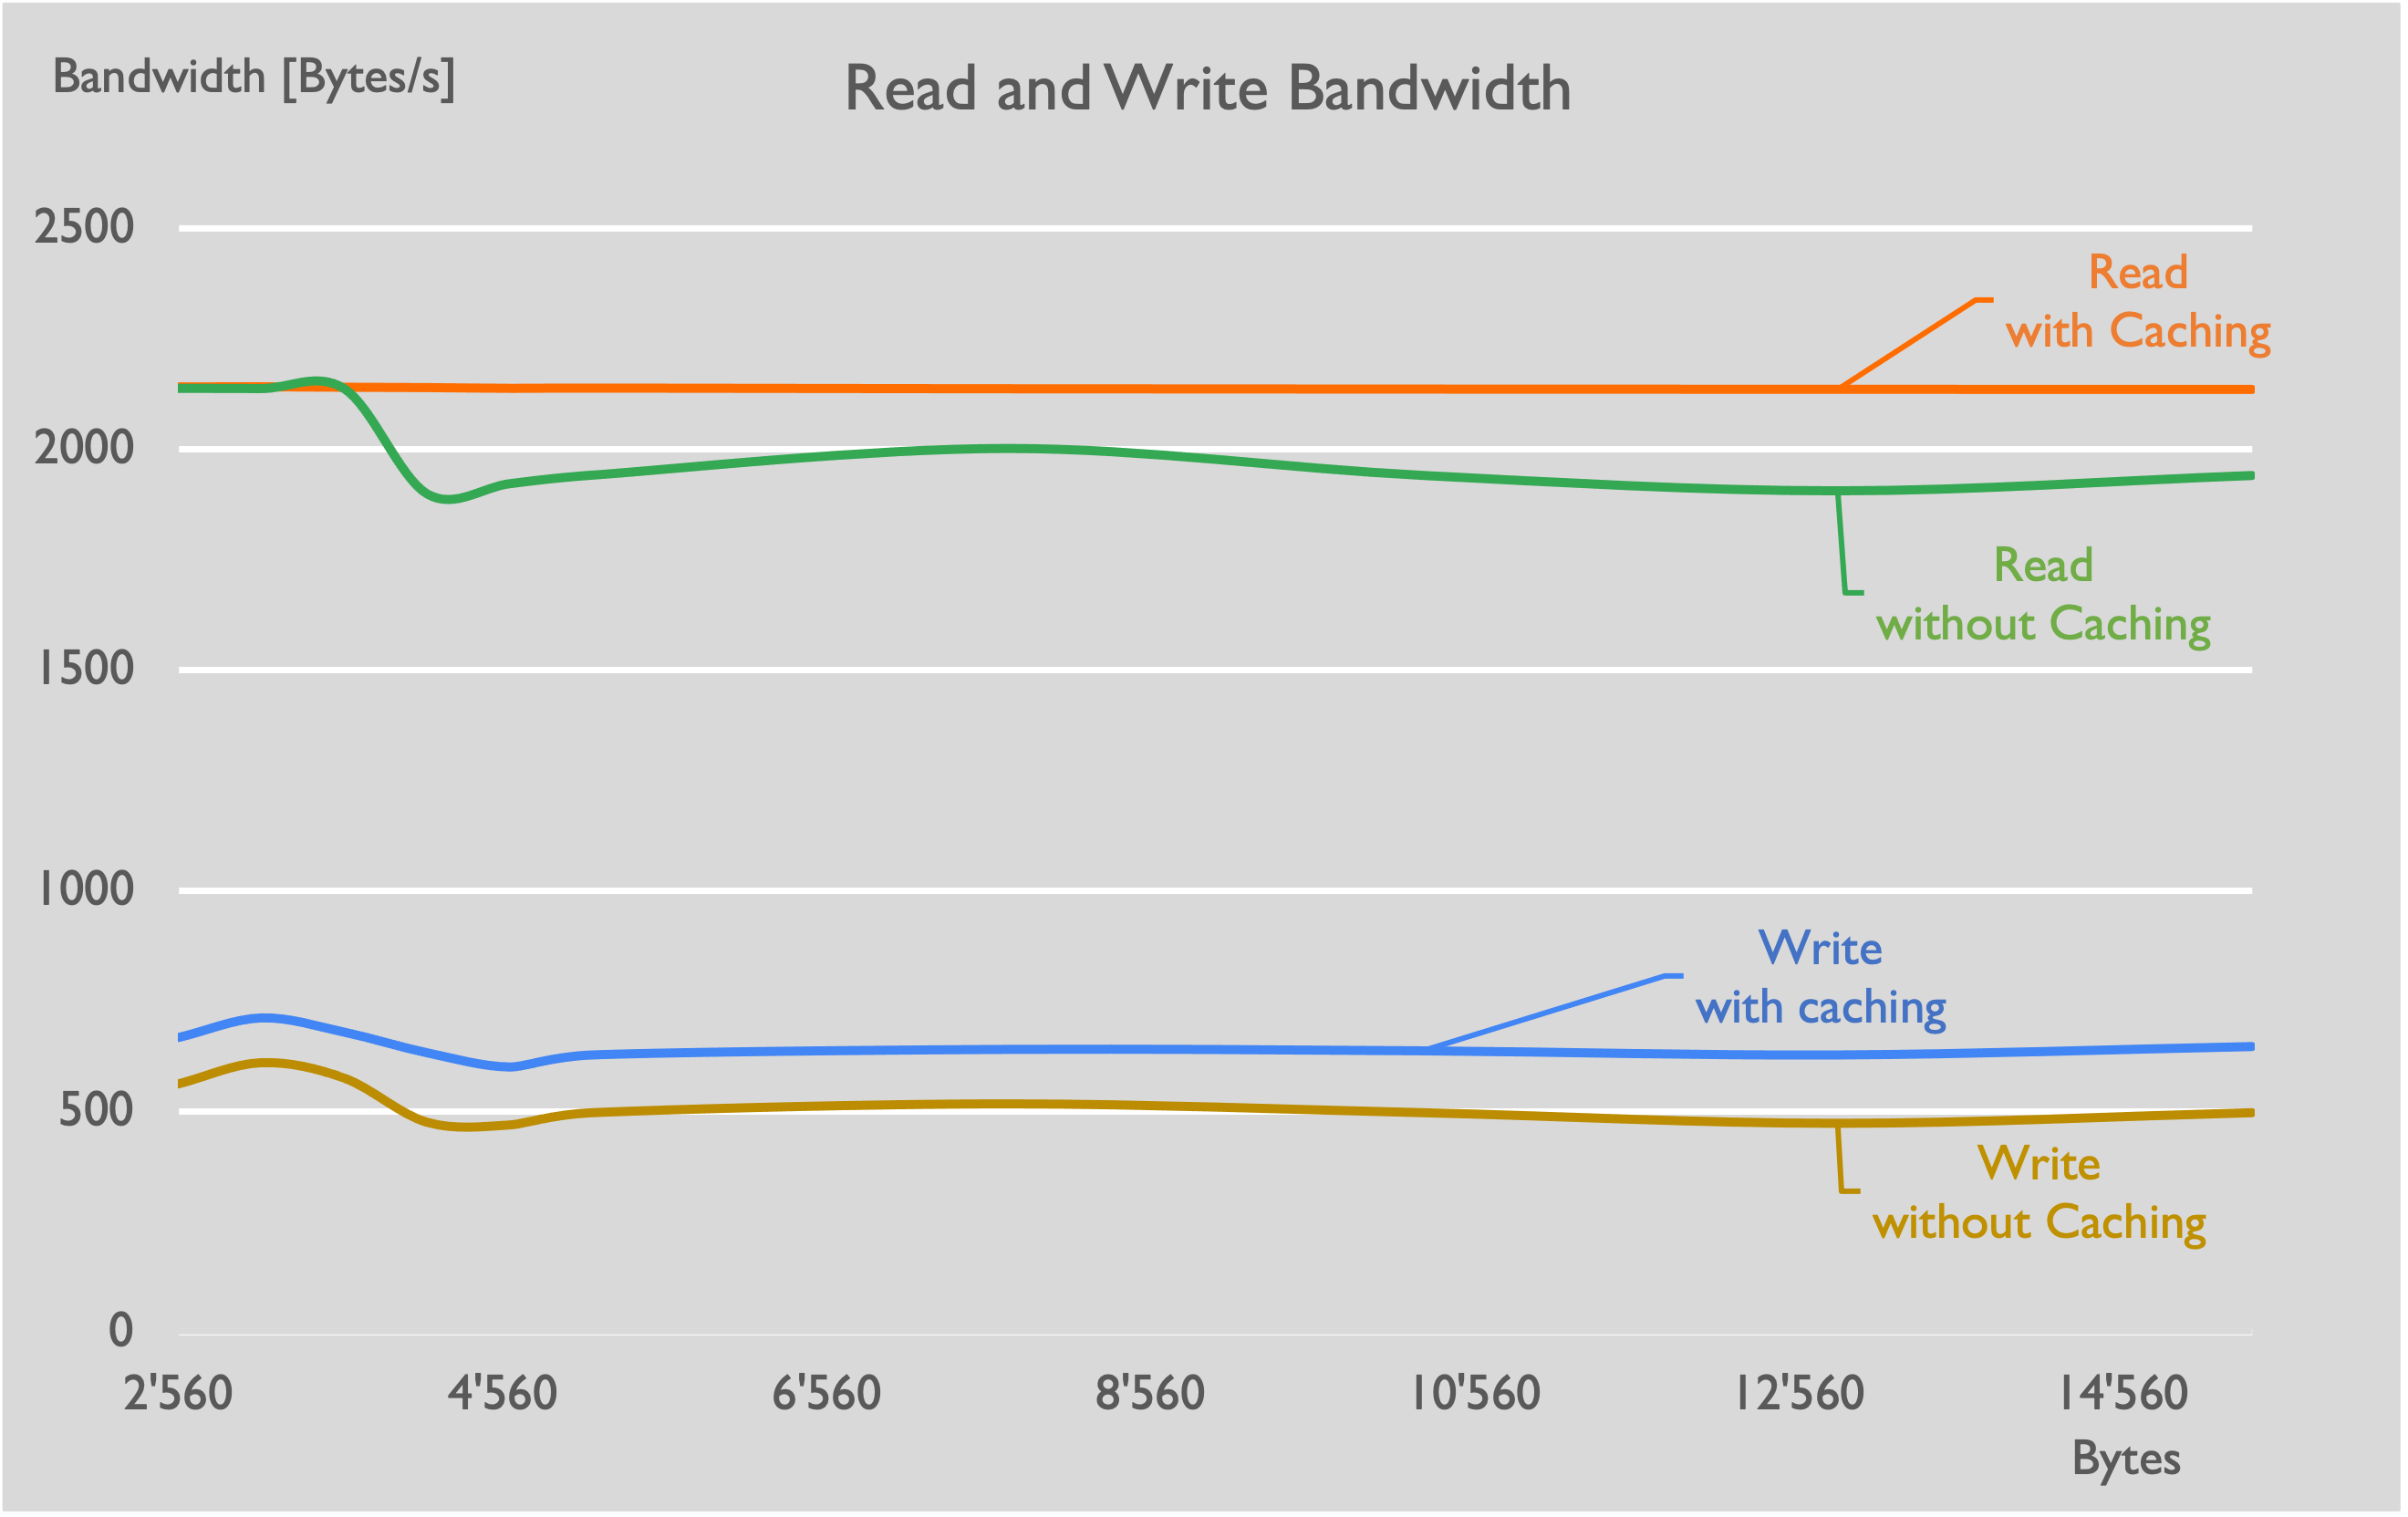
\includegraphics[scale=0.55]{fs_rw_new.png}
\caption{Read/Write Bandwidth with and without caching}
\label{fig:fs_rw_bw}
\end{figure}

In Figure~\ref{fig:fs_rw_bw}, we measured the read and write performance of our filesystem through a separate process which access the filesystem.
As you can see, the bandwidth stays very consistent in comparison with file sizes and we achieve a maximal read bandwidth of roughly 2.1KB/s,
which is very close to the block driver read bandwidth: 2.14KB/s. This can be explained by noting that in the sizes we have tested,
the FAT sector is cached all the time, so there is at most one read access for the FAT sector on which all of the read/write requests map to.
Thus, lookups to find next clusters in the linked list of clusters are near-instant, allowing the read-performance to be very close to the 
read-bandwidth of the block driver. If we look at the read-bandwidth of the filesystem without caching, it can be seen that now the FAT
sector needs to be looked up all the time, so performance drops there by roughly 250B/s, which is explained precisely by the additional read request into the 
FAT sector.

For writes, we are much lower as we now cannot make much use of the cached data, as write will always have to be performed. While the following reads
are still cached, we take a heavy toll because of those. Additionally, to keep the filesystem thread safe, after every RPC request for a write,
we update the directory entry with the new file size. Since the filesystem service is designed to write at most 1024 bytes per request, this 
furthermore gives use a 33\% overhead on the write bandwidth, as we have twice as many write requests.
Again, we see that caching still helps with the performance.


\section{Issues}
We already explained what features from the FAT32 specification are missing. Issues with the existing code are most of all
read performance, which is dominated by our slow RPC implementation. Continued work on this matter would be started there,
as it would resolve many performance problems.